\documentclass[a3shrink,landscape, final]{baposter}
%\documentclass[a4shrink,portrait,final]{baposter}
% Usa a4shrink for an a4 sized paper.

\tracingstats=2

\usepackage{times}
\usepackage{calc}
\usepackage{graphicx}
\usepackage{amsmath}
\usepackage{amssymb}
\usepackage{relsize}
\usepackage{multirow}
\usepackage{bm}

\usepackage{graphicx}
\usepackage{multicol}

\usepackage{pgfbaselayers}
\pgfdeclarelayer{background}
\pgfdeclarelayer{foreground}
\pgfsetlayers{background,main,foreground}

\usepackage{helvet}
%\usepackage{bookman}
\usepackage{palatino}

\newcommand{\captionfont}{\footnotesize}
\newcommand{\zebox}[1]{$|\underline{\overline{#1}}|$}

\selectcolormodel{cmyk}

\graphicspath{{images/}}

%%%%%%%%%%%%%%%%%%%%%%%%%%%%%%%%%%%%%%%%%%%%%%%%%%%%%%%%%%%%%%%%%%%%%%%%%%%%%%%%
%%%% Some math symbols used in the text
%%%%%%%%%%%%%%%%%%%%%%%%%%%%%%%%%%%%%%%%%%%%%%%%%%%%%%%%%%%%%%%%%%%%%%%%%%%%%%%%
% Format 
% \newcommand{\Matrix}[1]{\begin{bmatrix} #1 \end{bmatrix}}
% \newcommand{\Vector}[1]{\Matrix{#1}}
% \newcommand*{\SET}[1]  {\ensuremath{\mathcal{#1}}}
% \newcommand*{\MAT}[1]  {\ensuremath{\mathbf{#1}}}
% \newcommand*{\VEC}[1]  {\ensuremath{\bm{#1}}}
% \newcommand*{\CONST}[1]{\ensuremath{\mathit{#1}}}
% \newcommand*{\norm}[1]{\mathopen\| #1 \mathclose\|}% use instead of $\|x\|$
% \newcommand*{\abs}[1]{\mathopen| #1 \mathclose|}% use instead of $\|x\|$
% \newcommand*{\absLR}[1]{\left| #1 \right|}% use instead of $\|x\|$
% 
% \def\norm#1{\mathopen\| #1 \mathclose\|}% use instead of $\|x\|$
% \newcommand{\normLR}[1]{\left\| #1 \right\|}% use instead of $\|x\|$

%%%%%%%%%%%%%%%%%%%%%%%%%%%%%%%%%%%%%%%%%%%%%%%%%%%%%%%%%%%%%%%%%%%%%%%%%%%%%%%%
% Multicol Settings
%%%%%%%%%%%%%%%%%%%%%%%%%%%%%%%%%%%%%%%%%%%%%%%%%%%%%%%%%%%%%%%%%%%%%%%%%%%%%%%%
\setlength{\columnsep}{0.7em}
\setlength{\columnseprule}{0mm}


%%%%%%%%%%%%%%%%%%%%%%%%%%%%%%%%%%%%%%%%%%%%%%%%%%%%%%%%%%%%%%%%%%%%%%%%%%%%%%%%
% Save space in lists. Use this after the opening of the list
%%%%%%%%%%%%%%%%%%%%%%%%%%%%%%%%%%%%%%%%%%%%%%%%%%%%%%%%%%%%%%%%%%%%%%%%%%%%%%%%
\newcommand{\compresslist}{%
\setlength{\itemsep}{1pt}%
\setlength{\parskip}{0pt}%
\setlength{\parsep}{0pt}%
}


%%%%%%%%%%%%%%%%%%%%%%%%%%%%%%%%%%%%%%%%%%%%%%%%%%%%%%%%%%%%%%%%%%%%%%%%%%%%%%
%%% Begin of Document
%%%%%%%%%%%%%%%%%%%%%%%%%%%%%%%%%%%%%%%%%%%%%%%%%%%%%%%%%%%%%%%%%%%%%%%%%%%%%%

\begin{document}

%%%%%%%%%%%%%%%%%%%%%%%%%%%%%%%%%%%%%%%%%%%%%%%%%%%%%%%%%%%%%%%%%%%%%%%%%%%%%%
%%% Here starts the poster
%%%---------------------------------------------------------------------------
%%% Format it to your taste with the options
%%%%%%%%%%%%%%%%%%%%%%%%%%%%%%%%%%%%%%%%%%%%%%%%%%%%%%%%%%%%%%%%%%%%%%%%%%%%%%
% Define some colors
\definecolor{silver}{cmyk}{0,0,0,0.3}
\definecolor{yellow}{cmyk}{0,0,0.9,0.0}
\definecolor{reddishyellow}{cmyk}{0,0.22,1.0,0.0}
\definecolor{black}{cmyk}{0,0,0.0,1.0}
\definecolor{darkYellow}{cmyk}{0,0,1.0,0.5}
\definecolor{darkSilver}{cmyk}{0,0,0,0.1}

\definecolor{lightyellow}{cmyk}{0,0,0.3,0.0}
\definecolor{lighteryellow}{cmyk}{0,0,0.1,0.0}
\definecolor{lightestyellow}{cmyk}{0,0,0.05,0.0}

\definecolor{white}{cmyk}{0,0,0,0}
\definecolor{blue}{cmyk}{0.74,0.27,0,0}
\definecolor{lighterblue}{cmyk}{0.85,0.0,0.0,0.0}
\definecolor{lightestblue}{cmyk}{0.09,0,0,0}
\definecolor{borderblue}{cmyk}{0.74,0.27,0,0.4}
\definecolor{headerblue}{cmyk}{0.74,0.27,0,0.5}
\definecolor{bgblue}{cmyk}{0.9,0.5,0.1,0}
\definecolor{bgblue2}{cmyk}{0,0,0,0}
\definecolor{boxColor1}{cmyk}{0.1,0.05,0,0}


\definecolor{darkred}{cmyk}{0,1,1,0.4}
\definecolor{lightred}{cmyk}{0,0.4,0.4,0}

\definecolor{borderred}{cmyk}{0,0.9,0.8,0.3}



%%
\typeout{Poster Starts}
\background{
  \begin{tikzpicture}[remember picture,overlay]%
    \draw (current page.north west)+(-2em,2em) node[anchor=north west] {\includegraphics[height=1.1\textheight]{images/silhouettes_background}};
  \end{tikzpicture}%
}

\newlength{\leftimgwidth}
\begin{poster} { %poster options
  % Show grid to help with alignment
  grid=no,
  % Column spacing
  colspacing=1em,
  % Color style
%   bgColorOne=bgblue2,
%   bgColorTwo=bgblue,
%   borderColor=borderblue,
%   headerColorOne=headerblue,
%   headerColorTwo=lightestblue,
%   headerFontColor=white,
%   boxColorOne=white,
%   boxColorTwo=boxColor1,
  bgColorOne=bgblue2,
  bgColorTwo=bgblue,
  borderColor=borderred,
  headerColorOne=darkred,
  headerColorTwo=red,
  headerFontColor=white,
  boxColorOne=white,
  boxColorTwo=boxColor1,
  % Format of textbox
  textborder=roundedleft,
  % Format of text header
  eyecatcher=no,
  headerborder=open,
  headerheight=0.08\textheight,
  headershape=roundedright,
  headershade=shade-lr,
  headerfont=\Large\textsf, %Sans Serif
  boxshade=shade-lr,
  background=shade-tb,
%  background=plain,
  linewidth=2pt
  }
  % Eye Catcher
  {\includegraphics[width=8.5em]{images/daisy-logo}} % eye catcher for this poster. (eyecatcher=no above). If an eye catcher is present, the title is centered between eye-catcher and logo.
  % Title
  {\sf %Sans Serif
  %\bf% Serif
  Effective Caching of Shortest Paths for Location-Based Services}
  % Authors
  {\sf %Sans Serif
  % Serif
  Jeppe Rishede Thomsen\\
  {\large Paper accepted at the ACM SIGMOD 2012 conference}
  }
  %{\sf
  %\normalsize Department of Computer Science, Aalborg University}
  % University logo
  {% The makebox allows the title to flow into the logo, this is a hack because of the L shaped logo.
    \makebox[8em][r]{%
      \begin{minipage}{24em}
        \hfill
        
\includegraphics[height=5.5em]{images/PolyU_Logo_CMKY}
      \end{minipage}
    }
  }

  \tikzstyle{light shaded}=[top color=baposterBGtwo!30!white,bottom color=baposterBGone!30!white,shading=axis,shading angle=90]

  % Width of left inset image
     \setlength{\leftimgwidth}{0.78em+8.0em}

%%%%%%%%%%%%%%%%%%%%%%%%%%%%%%%%%%%%%%%%%%%%%%%%%%%%%%%%%%%%%%%%%%%%%%%%%%%%%%
%%% Now define the boxes that make up the poster
%%%---------------------------------------------------------------------------
%%% Each box has a name and can be placed absolutely or relatively.
%%% The only inconvenience is that you can only specify a relative position 
%%% towards an already declared box. So if you have a box attached to the 
%%% bottom, one to the top and a third one which should be in between, you 
%%% have to specify the top and bottom boxes before you specify the middle 
%%% box.
%%%%%%%%%%%%%%%%%%%%%%%%%%%%%%%%%%%%%%%%%%%%%%%%%%%%%%%%%%%%%%%%%%%%%%%%%%%%%%
    %
    % A coloured circle useful as a bullet with an adjustably strong filling
    \newcommand{\colouredcircle}[1]{%
      \tikz{\useasboundingbox (-0.2em,-0.32em) rectangle(0.2em,0.32em);
\draw[draw=black,fill=borderblue!80!black!#1!white,line width=0.03em] (0,0)
circle(0.18em);}}

    \newenvironment{indentpar}[1]%
    { \vspace{-1em}
      \begin{list}{}%
	    {\setlength{\leftmargin}{#1}}%
	    \item[]%
    }
    {\end{list} \vspace{-1em}}

%%%%%%%%%%%%%%%%%%%%%%%%%%%%%%%%%%%%%%%%%%%%%%%%%%%%%%%%%%%%%%%%%%%%%%%%%%%%%%
  \headerbox{Applications \& Objectives}{name=contribution,span=1.5,column=0,row=0}{
%%%%%%%%%%%%%%%%%%%%%%%%%%%%%%%%%%%%%%%%%%%%%%%%%%%%%%%%%%%%%%%%%%%%%%%%%%%%%%


	\begin{center}
	  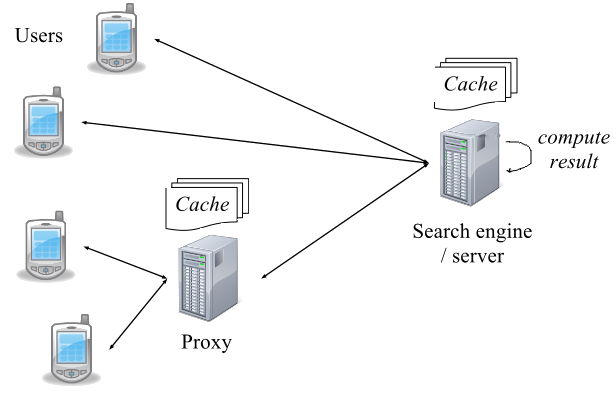
\includegraphics[width=0.60\linewidth]{images/scenario} 
	\end{center}

\colouredcircle{100} \textbf{Scenario:} Users submit shortest path queries to an online route service provider. A static cache is employed at either of two locations:

  \begin{indentpar}{0.5cm}
	  $-$ The server, to save shortest path calculation.

	  $-$ A proxy, to save network communication.
   \end{indentpar}


 \colouredcircle{100} \textbf{Applications:} A static cache to store shortest path query results. Applicable to all existing online shortest path service providers.

 \colouredcircle{100} \textbf{Motivation:} Online route service providers are becoming increasingly popular and shortest path calculation is expensive. %No work has been done on caching of shortest paths.

 \colouredcircle{100} \textbf{Objectives:} (1) To add the best Shortest Paths to the cache, (2) Introduce cache data structure to store the Shortest Paths efficiently.

  \vspace{0.5em}
 }



% 
% The cache storage structure is optimized so that each edge from the road network is only stored once in the cache. 
% 
%  \colouredcircle{100} \textbf{Experimental results:} The static cache is efficient; able to both save communication and shortest path calculation cost.
% 

%%%%%%%%%%%%%%%%%%%%%%%%%%%%%%%%%%%%%%%%%%%%%%%%%%%%%%%%%%%%%%%%%%%%%%%%%%%%%%
  \headerbox{Contributions}{name=questions,column=0,span=1.5,below=contribution,above=bottom}{
%%%%%%%%%%%%%%%%%%%%%%%%%%%%%%%%%%%%%%%%%%%%%%%%%%%%%%%%%%%%%%%%%%%%%%%%%%%%%%

\begin{center}
   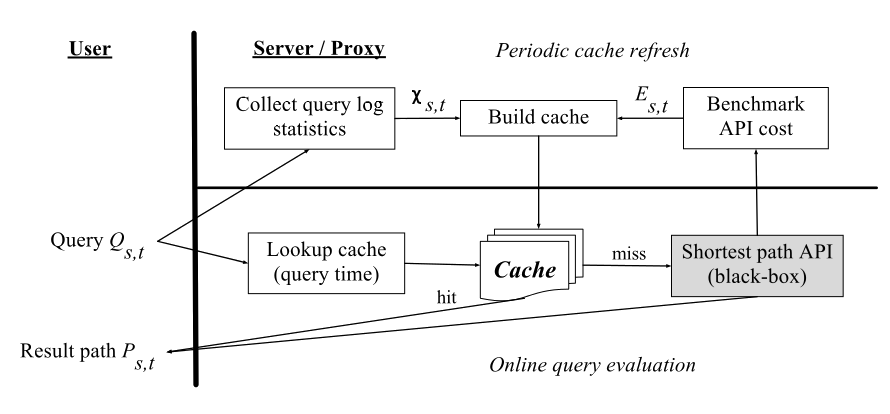
\includegraphics[width=0.85\linewidth]{images/routequery2}   
\end{center}

   \colouredcircle{100}  We formulate a systematic model for quantifying the benefit of caching a specific shortest path. \vspace{0.5em}

   \colouredcircle{100}  We design techniques for extracting statistics from query logs and benchmarking the cost of a shortest path call. \vspace{0.5em}

   \colouredcircle{100}  We propose an algorithm for selecting paths to be placed in the cache.\vspace{0.5em}

   \colouredcircle{100}  We develop a compact and efficient cache structure for storing shortest paths.\vspace{0.5em}

   \colouredcircle{100}  We study the above contributions empirically using real data.\vspace{0.5em}



% 
% The static cache content is build offline using (1) Historical query log statics ($\chi_{s,t}$), and (2) benchmark ($E_{s,t}$) of the cost of calculating a shortest path.
% 
% Below the horizontal line we introduce a transparent cache, not modifying anything in the existing service. Above the horizontal line we periodically recalculate the cache content and replace the online cache below the line.
}

%%%%%%%%%%%%%%%%%%%%%%%%%%%%%%%%%%%%%%%%%%%%%%%%%%%%%%%%%%%%%%%%%%%%%%%%%%%%%%
  \headerbox{Building the Cache for Shortest Paths}{name=incremental benefit,column=1.5,span=2.5,row=0}{
%%%%%%%%%%%%%%%%%%%%%%%%%%%%%%%%%%%%%%%%%%%%%%%%%%%%%%%%%%%%%%%%%%%%%%%%%%%%%%
  
%   \includegraphics[width=\linewidth]{images/dgDemo}

\begin{center}
\begin{tabular}{ccc}

\begin{tabular}{c}
\\
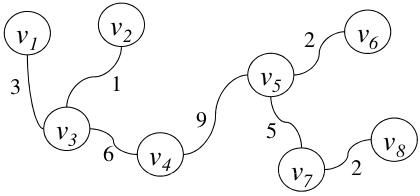
\includegraphics[width=0.30\linewidth]{images/rxmap}
\end{tabular}
&

\begin{tabular}{@{}|c@{}|c@{}|@{}}
\hline
Timestamp & Query \\ \hline 
$T_1$ & $Q_{3,6}$ \\ \hline 
$T_2$ & $Q_{1,6}$ \\ \hline 
$T_3$ & $Q_{2,7}$ \\ \hline 
$T_4$ & $Q_{1,4}$ \\ \hline 
$T_5$ & $Q_{4,8}$ \\ \hline 
$T_6$ & $Q_{2,5}$ \\ \hline 
$T_7$ & $Q_{3,6}$ \\ \hline  
$T_8$ & $Q_{3,6}$ \\ \hline 
\end{tabular}

&

\begin{tabular}{@{}|@{}c@{}||@{}c@{}|@{}c@{}|@{}c@{}|@{}c@{}|@{}c@{}|@{}c@{}||@{}c@{ }|@{}c@{ }|}\hline
    Round & \multicolumn{6}{c||}{ Path } & \multicolumn{2}{@{ }c@{ }|}{Cache $\Psi$ }  \\ \cline{2-9}
             	& $P_{1,4}$ & $P_{1,6}$ & $P_{2,5}$ & $P_{2,7}$ & $P_{3,6}$ &  $P_{4,8}$ & Before round & After round 	 	 \\\hline \hline
    1	&  1/3    & \zebox{\bf 5/5}	 & 1/4    & 2/5 &  3/4    & 1/4 &  empty    & $P_{1,6}$ \\\hline
    2	&  0    & 0 &  1/4    & \zebox{\bf 2/5} &  0    & 1/4 & $P_{1,6}$    & $P_{1,6}, P_{2,7}$  \\\hline
    3	&  0    & 0 &  0   & 0 &  0    & \zebox{\bf 1/4} & $P_{1,6}, P_{2,7}$    & $P_{1,6}, P_{2,7}, P_{4,8}$  \\\hline
\end{tabular} \\

 (a) & (b) & (c)\\
\end{tabular}
\end{center}


The cache is built by incrementally calculating the benefit of shortest path results (a) from a historical query log (b).

The benefit equation $\Delta\overline{\gamma}(P_{a,b}, \Psi) = \sum\limits_{P_{s,t} \in \mathfrak{U}(P_{a,b}) - \mathfrak{U}(\Psi)} \frac{\chi_{s,t} \cdot E_{s,t}}{|P_{a,b}|}$ is to used here to calculate the benefit of the cache.

{\tiny $P_{a,b}$: a shortest path. $\Psi$: the cache. $\mathfrak{U}(P_{a,b})$: all subsets of $P_{a,b}$. $\chi_{s,t}$ frequency of query $s$ to $t$. $E_{s,t}$: cost of calculating $P_{s,t}$}

For our example we use figure (a), a small road network, and table (b), a query log where $Q_{s,t}$ means a query from $s$ to $t$, as the basis for calculating the numbers in (c).

Table (c) illustrates the incremental calculation of shortest path benefits. Each unique path from query log (b) is illustrated in the Path column of (c). In the fractions the numerator represents the number of queries from (b), which can not already be answered by the cache, a path can answer. The denominator is the length of the path

\textbf{Round 1:} $P_{1,6}$ can answer $P_{1,4}, P_{1,6}$, and $P_{3,6}$. These tree queries appear 5 times in (b). $P_{1,6}$ is largest and added to the cache. 

\textbf{Round 2:} $P_{1,4}, P_{1,6}$, and $P_{3,6}$ are now all $0$ since adding them will not allow the cache to answer any additional queries. $P_{2,7}$ is added.

\textbf{Round 3:} $P_{4,8}$ is the only path left which can add benefit to the cache, so we add it. The algorithm terminates as there are no more paths which can provide additional benefit to the cache.

  \vspace{0.5em}
  }

%%%%%%%%%%%%%%%%%%%%%%%%%%%%%%%%%%%%%%%%%%%%%%%%%%%%%%%%%%%%%%%%%%%%%%%%%%%%%%
  \headerbox{Results}{name=results,column=1.5,span=2.5,above=bottom,below=incremental benefit}{
%%%%%%%%%%%%%%%%%%%%%%%%%%%%%%%%%%%%%%%%%%%%%%%%%%%%%%%%%%%%%%%%%%%%%%%%%%%%%%

\begin{center}
\begin{tabular}{ccc}
     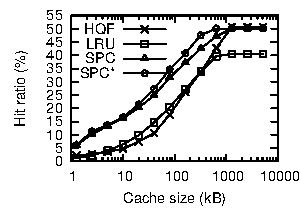
\includegraphics[width=0.3\linewidth]{images/cachesize_hitratio_bei.pdf}
&
     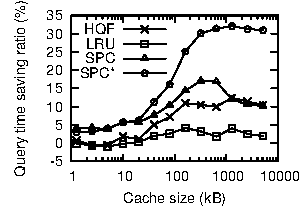
\includegraphics[width=0.3\linewidth]{images/cachesize_diffruntime_bei_server.pdf}
&
     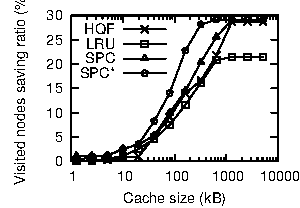
\includegraphics[width=0.3\linewidth]{images/cachesize_diffnodes_bei_server.pdf}
\\
 (a) & (b) & (c)\\
\end{tabular}
\end{center}

Our approach was evaluated using GPS traces in two large cities, Beijing \& Aalborg. The endpoints were extracted to build a query log. For our experiments the log was equally divided into a historical query log and workload queries. Above in (A)-(C) the results from Beijing is shown. We compare our selves against two competitors \textit{Least Recently Used (LRU)} and \textit{Highest Query Frequency (HQF)}. Our method is SPC, which we test with two different cache representations. LRU, HQF, and SPC all use an inverted list to represent the cache, while SPC$^*$ use a form of prefix compression, allowing for many more cache items in the cache, given the same cache size.

In figure (a) we test the hit ratio for varying cache sizes. This measure is important for our Proxy scenario, where the goal is to save reduce network communication with the server. A higher hit ratio will be directly correlated to less network traffic to the server. 

In figure (b)/(c) we measure the percentage of time and vertices's involved in shortest path calculation, which we can save/avoid compared to not using any caching.

  \vspace{0.5em}
 }

\end{poster}%
\end{document}
